\documentclass[11pt,a4paper]{article}
\usepackage{jheppub}
\usepackage{amssymb}
\usepackage{amsmath}
\usepackage{graphicx}
\newcommand{\expval}[1]{\left\langle#1\right\rangle}
\newcommand{\dd}{\mathrm{d}}

\title{One-loop effective action for the average Ising magnetization on compact manifolds}
\author{Andrea Allais}
\emailAdd{allais.andrea@gmail.com}

\begin{document}

\maketitle

\section{Main results}

The average magnetization $\bar{\phi} = \frac{1}{V} \sum_{i} \sigma_i$ of the
Ising model is the simplest observable in Monte Carlo simulations. For large
system size, the probability distribution of $\bar{\phi}$ changes qualitatively
between the two phases of the model. In the symmetric phase, if the
correlation length $\xi$ is large in lattice units, but small compared to the
system size $R$, the distribution is well approximated by a unimodal Gaussian
centered at 0. In the broken symmetry phase, still for $1 \ll \xi \ll R$, the
distribution is well approximated by a bimodal superposition of two 
Gaussians centered at non-zero values $\pm \bar{\phi}_0$. 

Near the critical point $1 \ll R \ll \xi$ the probability distribution is a
non-trivial function of $\bar{\phi}$, at least in two and three dimensions.  It
is not immediately clear if the same is true in four dimensions as well.  Since
the $\phi^4$ field theory that describes the Ising critical point in four
dimensions becomes weakly coupled in the infrared, one may expect the
probability distribution to be a Gaussian at the critical point as well.

To clarify this issue, we compute the one-loop effective action, or log
probability, for $\bar{\phi}$ in $4$ dimensions, and show that for
very large system size, the critical probability distribution is not Gaussian,
but rather of the form $p(\bar{\phi})\sim \exp(-a \bar{\phi}^4)$. We find that
corrections to this form vanish very slowly with increasing system size, like
$1/\log R$.

Thus we consider the $\phi^4$ field theory:

\begin{equation}
  S[\phi] = \int_{\mathcal{M}}\left(
    \frac{1}{2} \phi\left(\Delta + r_0\right)\phi +
    \frac{1}{2} \xi_0 \phi^2 \mathcal{R} +
    \frac{1}{24} u_0 \phi^4\right)
\end{equation}

on both the 4-torus $\mathcal{M} = S_1^4$ or the 4-sphere $\mathcal{M} = S_4$.
Here $\mathcal R$ denotes the scalar curvature. We define the effective action:

\begin{equation}
  e^{-S_{\mathrm{eff}}(\bar\phi)} = \int \left[\mathcal{D}\phi\right]
    \delta\left(\bar{\phi} - \frac{1}{V}\int_{\mathcal{M}}\phi\right)
    e^{-S[\phi]}\,,
\end{equation}

and we obtain:

\begin{equation}
\label{eq:effective_action}
\begin{split}
  \frac{S_{\mathrm{eff}}(\bar{\phi})}{V} = 
  &\frac{1}{2} \frac{\bar{\phi}^2}{R^2} \left(
    r R^2 + \eta + \frac{g}{6} f_1\left(r R^2 + \eta\right)
    + O\left(g^2\right)\right) + \\
  & \frac{2\pi^2}{9}g\bar{\phi}^4\left(
    1 - \frac{g}{2}f_2\left(r R^2 + \eta\right)
    + O\left(g^2\right)\right) + \\
  & \frac{8\pi^4}{81} g^3 \bar{\phi}^6 R^2\left(
    f_3\left(r R^2 + \eta\right)
    + O\left(g\right)\right) + O\left(g^4\bar{\phi}^8\right)\,,
\end{split}
\end{equation}

where $R$ is the radius of either manifold, and the coefficients
$(r,\,\eta,\,g)$ are the renormalized counterparts to $(r_0,\,\xi,\,u_0)$. An
explicit expression for the functions $f_1$, $f_2$ and $f_3$ is reported in the
appendix (\ref{eq:f_functions}), and they are plotted in
fig.~\ref{fig:f_functions}.

\begin{figure}
\begin{center}
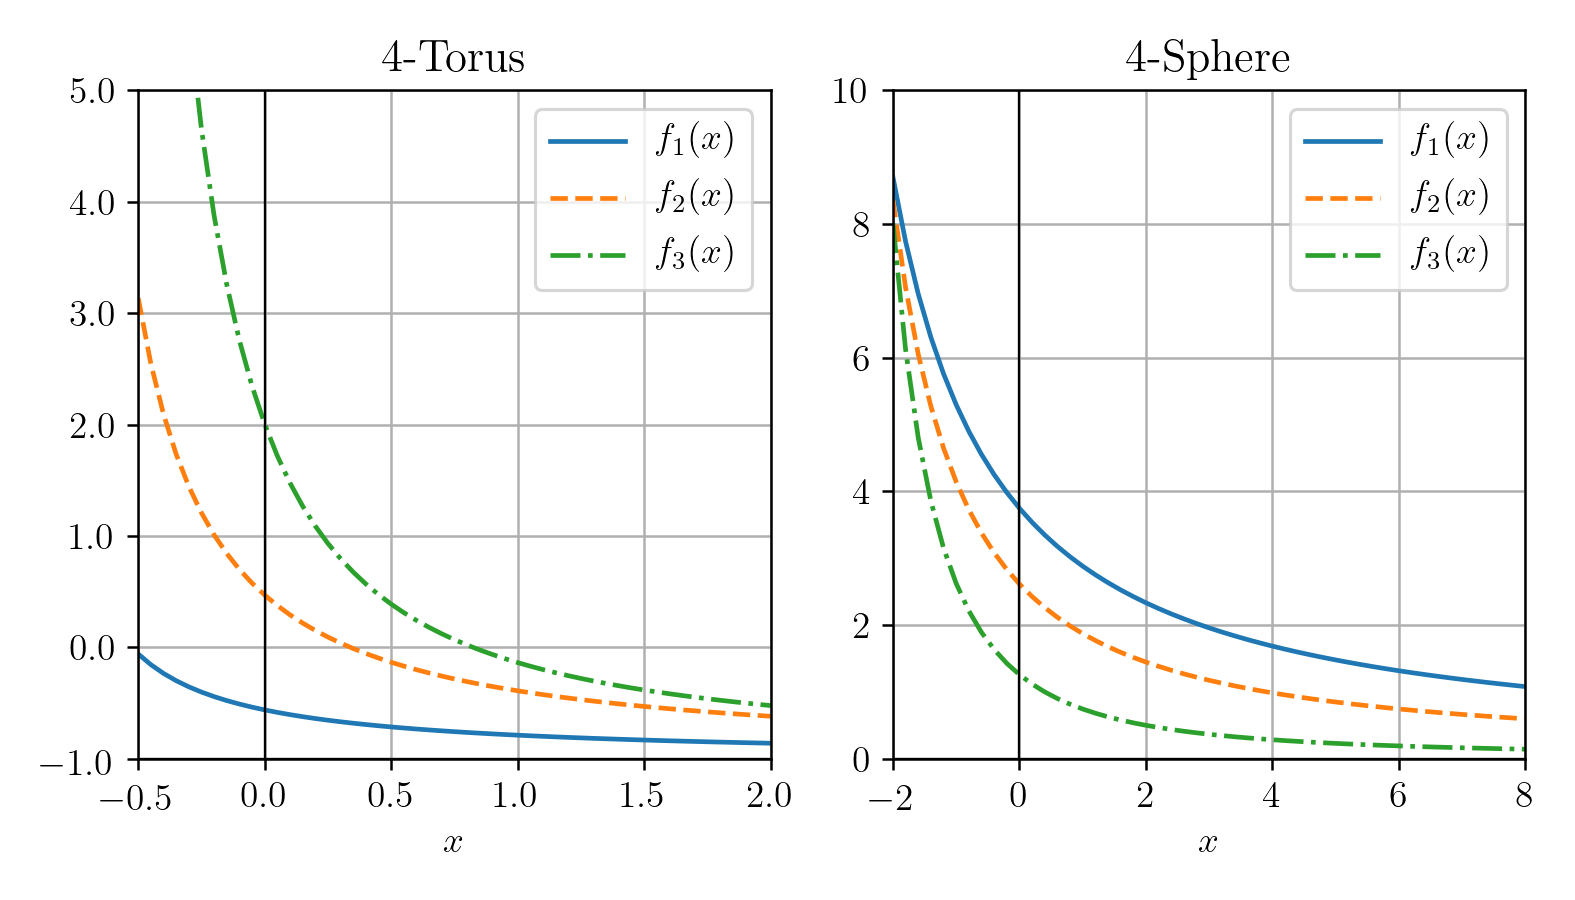
\includegraphics{f_functions.png}
\end{center}
\caption{\label{fig:f_functions} The functions $f_i$}
\end{figure}

This is our central result, and we will now describe it at lenght, beginning
with its domain of validity and its dependence on the couplings on a manifold
of fixed radius $R$.

The coupling $\eta$ is the counterpart to the curvature coupling
$\xi_0$, and hence is exactly zero for the torus, whereas it is a free,
dimensionless parameter for the sphere.

The dimension-2 coupling $r$ controls the cross-over between the symmetric and
broken-symmetry phases. The expression (\ref{eq:effective_action}) is valid for
$r R^2 + \eta \gtrsim -1$. It becomes invalid for lower values of $r$ because
the condensation of higher modes of the laplacian invalidates the perturbative
expansion. This becomes manifest in a divergence of the functions $f_i$ as
their argument approaches -1 for the torus, or  -4 for the sphere.  On the
other hand, $f_1$, $f_2$, $f_3$ remain finite as their argument approaches
positive infinity, and hence for large $r$ the probability distribution of
$\bar{\phi}$ is a Gaussian:

\begin{equation}
  \frac{S_{\mathrm{eff}}(\bar{\phi})}{V} \sim \frac{1}{2} r \bar{\phi}^2
  \quad \text{for} \quad
  rR^2 \gg 1\,.
\end{equation}

The dimensionless coupling $g$ is the parameter of the perturbative expansion.
The expansion is valid for $g \ll 1$, provided $rR^2$ is sufficiently far from
the bound discussed above.



In general,
they depend on a renormalization scale $\mu$, and it is possible to derive an
expression for $S_{\mathrm{eff}}$ evaluated at a generic value of $\mu$. Here,
for simplicity we choose to evaluate (\ref{eq:effective_action}) at the scale
$\mu^2 = r + p^2$. This value of $\mu$ is optimal for the reliability of
perturbation theory, because it avoids the emergence of large logarithms.

  As is well
known, in $4 - \varepsilon$ dimensions it satisfies the renormalization group
equation:

\begin{equation}
  \mu \frac{\dd g}{\dd \mu} = -\varepsilon g + g^2\,.
\end{equation}

The Wilson-Fisher fixed point is attained at $g_{\star} = \varepsilon$, and
substituting $g \to \varepsilon$ in (\ref{eq:effective_action}) and dropping
higher order terms in $\varepsilon$ yields the effective action at the fixed
point to leading order in $\epsilon$.

The coupling $r$ satisfies the renormalization group equation:
\begin{equation}
  \mu \frac{\dd r}{\dd \mu} = \frac{g}{3}r
\end{equation}

$r$, $\eta$, and $g$ are renormalized couplings
that satisfy the renormalization group equations:

\begin{align}
  &\mu \frac{\dd g}{\dd \mu} = -\varepsilon g + g^2 \\
  &\mu \frac{\dd r}{\dd \mu} = \frac{g}{3}r \\
  &\mu \frac{\dd \eta}{\dd \mu} = \frac{g}{3}(\eta - 2)
\end{align}

The coupling $\eta$ is related to the coupling between the scalar and
the curvature, and hence it is exactly zero on the tourus. On the sphere, it
may seem that it can be set to a constant value $\eta = 2$ at all energy
scales, however this ceases to be true at higher orders in perturbation theory,
where the renormalization group equation becomes inhomogeneous.

While a general expression for the effective action at a generic scale $\mu$ is
available, for simplicity (\ref{eq:effective_action}) is evaluated at $\mu^2
= r + p^2$. This value of $\mu$ is optimal for the reliability of perturbation
theory, because it minimizes the effect of the so-called large logs.

An explicit expression for the functions $f_1$, $f_2$, $f_3$ is reported in the
appendix. As shown in fig.~\ref{fig:f_functions}, $f_i(x)$ is of order 1 in for
$x \gtrsim -1/2$, $f_1$ approaches a constant as $x \to \infty$, whereas
$f_2$ and $f_3$ approach 0. They all diverge as $x$ approaches $-1$.
\section{Appendix}


\begin{equation}
\label{eq:f_functions}
f_1 = 
\end{equation}
\end{document}
